\documentclass[11pt,reqno]{amsart}

\setlength{\textheight}{8.8in}
\setlength{\topmargin}{-.1in}
%\setlength{\textwidth}{6in}
%\setlength{\oddsidemargin}{.26in}
%\setlength{\evensidemargin}{.26in}
\parskip=.08in

\usepackage[pagebackref]{hyperref} % for pdflatex
%\usepackage[hypertex,pagebackref]{hyperref} % for latex
\usepackage{xcolor}
\usepackage{amsmath,amsthm}
\usepackage{amssymb}
\usepackage{graphicx}
\usepackage[mathscr]{eucal}
\usepackage{MnSymbol}
\usepackage[frame,ps,matrix,arrow,curve,rotate,all,2cell,tips]{xy}
\usepackage{enumerate}

\setcounter{tocdepth}{1}

% The second argument here is about how to label the theorems, e.g. Theorem 2.2 is the second thing in section 2. The first thing in section 2 is subsection 2.1.
\newtheorem{theorem}[subsection]{Theorem}
\newtheorem{lemma}[subsection]{Lemma}
\newtheorem{sublemma}[subsection]{Sub-Lemma}
\newtheorem{proposition}[subsection]{Proposition}
\newtheorem{corollary}[subsection]{Corollary}
\newtheorem{thm}[subsection]{Theorem}
\newtheorem{prop}[subsection]{Proposition}



%%% The following environments have roman body.

\theoremstyle{definition}
\newtheorem{definition}[subsection]{Definition}
\newtheorem{example}[subsection]{Example}
\newtheorem{remark}[subsection]{Remark}
\newtheorem{assumption}[subsection]{Assumption}
\newtheorem{convention}[subsection]{Convention}
\newtheorem{notation}[subsection]{Notation}
\newtheorem{conjecture}[subsection]{Conjecture}
\newtheorem{construction}[subsection]{Construction}
\newtheorem{work}[subsection]{Just For Us}

\numberwithin{equation}{subsection}

%\newtheorem{defn}[subsubsection]{Definition}
% donald has this command reserved
\newtheorem{conj}[subsection]{Conjecture}
\newtheorem{fact}[subsection]{Fact}
\newtheorem{problem}[subsection]{Problem}

% Common number systems
\renewcommand{\P}{\mathbb{P}}
\newcommand{\N}{\mathbb{N}}
\newcommand{\bbP}{\mathbb{P}}
\renewcommand{\H}{\mathbb{H}}

\newcommand{\Q}{\mathbb{Q}}
\newcommand{\R}{\mathbb{R}}
\newcommand{\Z}{\mathbb{Z}}
\newcommand{\F}{\mathbb{F}}

\renewcommand{\O}{\mathsf{O}}
\newcommand{\bbA}{\mathbb{A}}
\newcommand{\bbC}{\mathbb{C}}
\newcommand{\bbG}{\mathbb{G}} % Additive/Multiplicative group
\newcommand{\G}{\mathbb{G}} % Additive/Multiplicative group

%\newcommand{\balpha}{\mathbb{\upalpha}}
%\newcommand{\bmu}{\mathbb{\upmu}}



















\begin{document}

\title{Self-Tuning Clustering: An Adaptive Clustering Method for Transaction Data}

\author{Haley Nugent, Taylor Heilman}


\maketitle

%===================
\section{Introduction}
%===================

Database mining has wide applications for improving marketing strategies. To improve these marketing strategies, we use data clustering. Data clustering divides a set of data items into separate groups such that items in the same group are as similar to one another as possible. Clustering large datasets can uncover useful patterns among the data.  Data clustering is commonly used by companies such as Amazon.  By identifying items frequently bought together, Amazon can advertise similar items to customers, increasing the chances of a customer seeing an item they want and buying it.

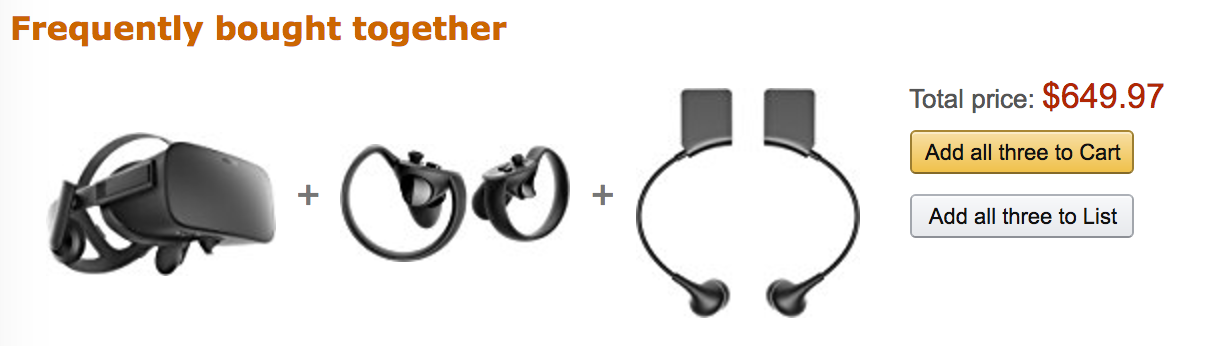
\includegraphics[scale=.5]{amazon}

Market-basket data is known to have high dimensionality, sparsity, and to have massive outliers. High dimensional data is a dataset with a large amount of attributes, often represented by large dimensional matrices. The data is known to have sparsity because there are many empty areas within the date. The outliers within the data can occur if certain items are hugely popular or hugely unpopular in comparison with the rest of the dataset.  The {\em small-large (SL) ratio} is the ratio of the number of small items to large items in the data.  A {\em large item} is an item which occurs frequently in transactions. A {\em small item} is an item that occurs infrequently in transactions. Smaller SL ratios indicate more similarity between the items in the cluster. This paper develops a {\em Self-Tuning Clustering algorithm (algorithm STC)} to efficiently cluster the market-basket data by adaptively tuning the SL ratio. The algorithm consists of three phases:
	\begin{enumerate}
		\item {\em pre-determination}: calculates the {\em minimum support S} and the {\em maximum ceiling E} according to a given parameter called {\em SL distribution rate $\beta$}.
		
		\item {\em allocation}: Algorithm STC uses the minimum support S to identify the large items. It uses the maximum ceiling E to identify the small items. It accomplishes this by scanning the database and allocating each transaction to a cluster for minimizing the SL ratio.
		
		\item {\em refinement}: Each transaction is evaluated to minimize its SL ratio in its corresponding cluster. 
	\end{enumerate}
	
	The algorithm uses two different kinds of SL ratio thresholds to evaluate the quality of the clustering, {\em output SL ratio threshold $\alpha^o$} and {\em input Sl ratio threshold $\alpha^i$}. A transaction is moved from one cluster to the excess pool if its SL ratio is larger than $\alpha^o$ and moved from the excess pool to one cluster is the SL ratio is smaller than $\alpha^i$.
	
Algorithm STC significantly improves the clustering quality for synthetic and real market-basket data. 


%==================================
\section{Problem Description}
%==================================

The market-basket data is represented by a set of transactions $D = {t_1, t_2, ..., t_h}$, where $D$ is the database holding the set of transactions. Each transaction $t_i$ is a set of items ${i_1, i_2,...,i_h}$. A clustering $U =< C_1, C_2, ..., C_k>$ is a partition of transactions where $C_i$ is a cluster consisting of a set of transactions. The minimum support $S$ and the maximum ceiling $E$ are determined according to the SL distribution rate $\beta$ in the pre-determination phase. 

\subsection{Large Items and Small Items}


$Sup_C(i)$ is the support of an item $i$ in a cluster $C$. The support of an item is defined as the percentage of transactions which contain item $i$ in cluster $C$. If $Sup_C(i)$ is larger than the minimum support $S$, the item $i$ in a cluster $C$ is  called a {\em large item}. If an item $j$ in a cluster $C$ has a $Sup_C(j)$ that is smaller than the maximum ceiling $E$ the item $j$ is called a {\em small item}. An item is called a middle item if it is neither large or small.

$\newline$

\centerline{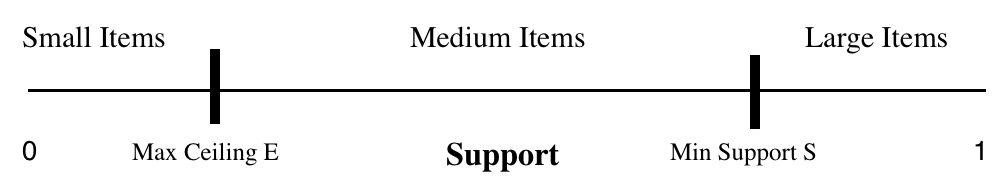
\includegraphics[scale=.5]{line}}


\subsection{Small-Large (SL) Ratio}

There are three kinds of SL ratios that need to be calculated in the data clustering procedure.
	\begin{enumerate}


	\item \textbf{SL Ratio of a Transaction:} The SL ratio for a transaction $t$ in cluster $C_i$ is defined as:
	$$R_{SL}(C_i, t) = \frac{|S(C_i,t)|}{|L(C_i, t)|} ,$$
$|S(C_i,t)|$ represents the number of small items in $t$ and $|L(C_i,t)|$ represents the number of large items in $t$.


	\item \textbf{SL Ratio of a Clustering:} The SL ratio for a clustering $U$ = $<C_1, ..., C_p>$ is defined as:
	$$R_{SL}(U) = \sum_{i=1}^{p} \sum_{j=1}^{N^T(C_i)} R_{SL}(C_i, t_j), $$
	$N^T(C_i)$ is the number of transactions and $t_j$ is the $j$th transaction in the cluster $C_i$. Essentially, we sum up the SL Ratio of a transaction for all transactions within an individual cluster. We then do this for every cluster within the clustering.
	
	
	
	\item \textbf{Average SL Ratio:} The average SL ratio for a clustering $U$ = $<C_1, ..., C_p>$ is defined as:
	$$\alpha(u) = \frac{R_{SL}(U)}{N^T(U)}$$
	 $N^T(U)$ is the number of transactions in clustering $U$. By dividing the SL Ratio of a Clustering by the number of transactions in the clustering, we can compute the average SL Ratio of the clustering.
	
	\end{enumerate}

\subsection{The Objective of Clustering Market-Basket Data}

{\em Given a database of transactions, determine a clustering U such that the average SL ratio $\alpha(U)$ is minimized.}  The clustering technique aims to maximize both the {\em intra-cluster similarity} and the {\em inter-cluster dissimilarity} of the data in order to minimize the average SL ratio. 

\textbf{Intra-Cluster Similarity:} Intra-Cluster Similarity of transactions means the transactions within a cluster are as similar to one another as possible. We achieve Intra-Cluster Similarity by maximizing the number of large items in each cluster while minimizing the number of small items in each cluster. We know that an item $i$ is large if there are relatively many transactions containing $i$, while an item $j$ is small if there are relatively few transactions containing $j$. Transactions are similar to one another if the contain many common large items and fewer small items. Thus, by maximizing large items in a cluster we construct a cluster with many similar transactions.

\textbf{Inter-Cluster Dissimilarity:} We achieve inter-cluster dissimilarity of transactions by maximizing the number of large items and minimizing the number of small items so dissimilar transactions will be allocated to the different clusters. Ideally, if an item $i$ is large in a cluster $C_a$, $i$ should be small in cluster $C_b$. 

%==================================
\section{Algorithm STC for Adaptively Clustering Market-Basket Data}
%==================================
 By utilizing the three SL ratios detailed in the previous section, Algorithm STC can efficiently and accurately cluster market-basket data. The defining factor which  makes Algorithm STC outperform other clustering algorithms is its self tuning technique, which adaptively tunes both the input and output SL ratio thresholds for iteratively minimizing $\alpha(U)$ (the average SL ratio). Algorithm STC is broken into three phases: the pre-determination phase, the allocation phase, and the refinement phase.

\subsection{The pre-determination phase}The pre-determination phase calculates minimum support $S$ and the maximum ceiling $E$, which are used later to determine whether an item is considered large, small or medium. The minimum support $S$ and the maximum ceiling $E$ are obtained by calculating the support of every item and then identifying related items according to the SL distribution rate $\beta$.  Recall that the support of an item is defined as the percentage of transactions which contain this item $i$ in cluster $C$. Explicitly, Algorithm STC counts the supports of items by scanning the database and then sorts the items according to their supports. We let $Count(\beta)$ be defined as the value $N^I$x$\beta$ where  $N^I$ represents the total number of items. Then, in the sorted list of items we let the minimum support $S$ = the support of the item whose support value is the $Count(\beta)^{th}$ largest.  Similarly, we let the maximum ceiling $E$ = the support of the item whose support value is the $Count(\beta)^{th}$ smallest. 

\subsection{The allocation phase} Once the minimum support $S$ and maximum ceiling $E$ are calculated the allocation phase begins. In the allocation phase STC determines the initial clustering $U_0$ for each transaction. Then, each transaction is read in sequence and is either assigned to an existing cluster or a new cluster is created and the transaction is assigned to said cluster. The objective in this phase is to minimize the SL ratio when assigning transactions to clusters.  We define $N_C$ as the current number of clusters and $\mu$ as the upper bound of the number of clusters allowed. Specifically, STC reads each transaction $t$ from database $D$. In the case that $N_C < \mu$ (we have yet to reach our maximum number of clusters) STC can either assign a transaction to an existing cluster or create a new cluster and assign the transaction to it. STC decides which option to choose by checking the $R_{SL}(C_i,t)$ (the SL Ratio of a Transaction). Transaction $t$ is assigned to an existing cluster $C_i$ if  $R_{SL}(C_i,t)$ is the minimum value compared to other clusters and $R_{SL}(C_i,t) < 1$. Otherwise, a new cluster is made, $t$ is assigned to the new cluster and $N_C$ is increased by one. In the case that $N_C = \mu$ (we've reached the maximum number of clusters allowed), $t$ is assigned to an existing cluster $C_i$ so that $R_{SL}(C_i,t)$ is the smallest. After all transactions are allocated to the clusters, STC obtains the initial clustering $U_0 =< C_1 , C_2 , ..., C_{N_C} >$ and the allocation phase is complete.

\subsection{The refinement phase}The self-tuning technique is exhibited in the refinement phase. After the initial cluster $U_0$ is created, STC then tunes the input ($\alpha ^i$) and output ($\alpha ^o$) SL ratio thresholds. First, STC identifies the large, middle and small items in each cluster using the minimum support $S$ and maximum ceiling $E$. In the first iteration STC sets $\alpha_1 ^o = \alpha_1 ^i = \alpha(U_0).$ So the both the input and output Sl ratio thresholds are set to equal to the average SL ratio. Then all transactions whose SL ratios are larger than $\alpha_1 ^o$ are moved to the excess pool. Note that the transactions in the excess pool are referred to as $excess$ $transactions$. Then STC creates an intermediate clustering $U_1^ \prime$ which does not contain the excess transactions. Algorithm STC again calculates the supports of items and identifies the large, middle and small items in each cluster found in $U_1^ \prime$. Then, for each excess transaction t, algorithm STC calculates its SL ratio in each cluster.  For transaction $t \in$ excess pool, if the smallest SL ratio of $t$ is in cluster $C_j$ and the Sl ratio is smaller than $\alpha_1 ^i$, then $t$ is moved from the excess pool to cluster $C_j$. Essentially, in this phase STC is finding the transactions who have poor Sl ratios in their current cluster. Then, STC finds the cluster that minimizes the SL ratio of each transaction in the excess pool.  If the minimum SL ratio of the current transaction is smaller than the minimum allowed SL ratio ($\alpha^i$) then the transaction is moved from the excess pool to its new cluster. In each subsequent iteration, STC starts with the clustering found in the previous iteration, adaptively tunes input and output SL ratio thresholds, and then re-clusters the transactions in the clustering and the excess pool. The procedure continues until no further movement is required (i.e., the average SL ratio $\alpha(U)$ cannot be reduced any more).


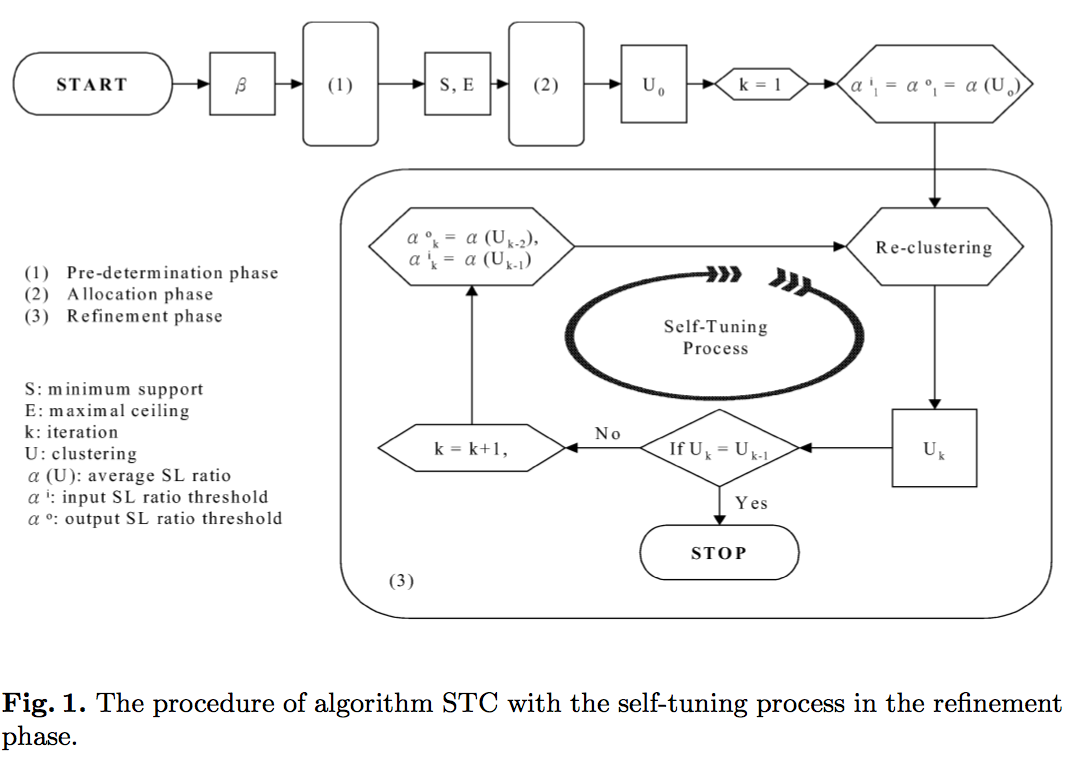
\includegraphics[scale=.70]{pic4}

%==================================
\section{Results}
%==================================
To accurately compare other Clustering algorithms with STC four experiments were conducted. Algorithm STC was compared to algorithm ROCK, algorithm SLR and algorithm STC without self-tuning techniques (referred to as Basic). Real data sets from the United States Congressional Votes records in 1984 containing 435 records were used in the experiments for performance evaluation. Each record contains 16 binary attributes corresponding to each congressman's vote on 16 issues. To provide further insight, synthetic data was generated for performance evaluation. The data was generated using the IBM Quest Synthetic Data Generation Code. This code generates transaction data which mimics the real world environment. In addition, real market-basket data from a large bookstore company is used, containing $|D| = 98934$ transactions and $N^I$ = 58909 items.

\subsection{Experiment One: Evaluating clustering quality for congressional voting data.}

The quality of each algorithm is evaluated by \textit{noise ratios}. The noise ratio is calculated by dividing the number of obscure politics in the clustering by the total number in the clustering. The smaller the noise ratio, the better the quality of the algorithm has.


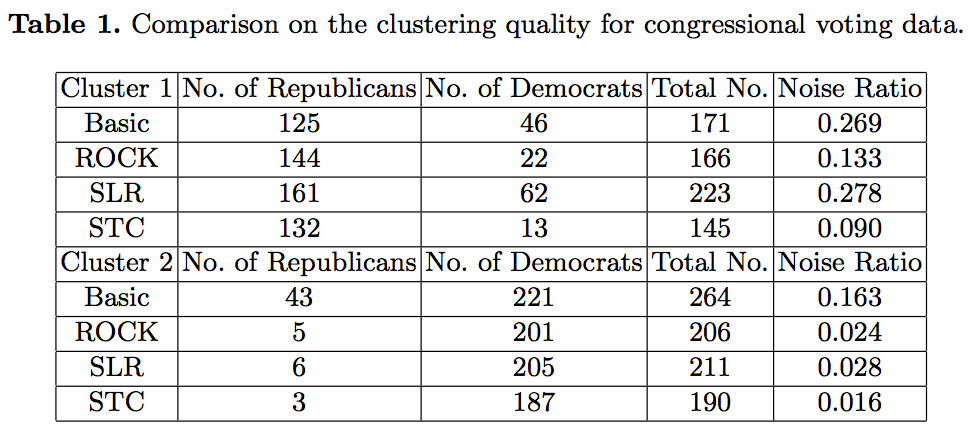
\includegraphics[scale=.75]{pic1}


As you can see from the results, STC with tuning-techniques emerged as the best quality out of all clustering algorithms.


\subsection{Experiment Two: Evaluating the clustering quality of issues for congressional voting data.} 

For each issue in the Congressional Voting records, each congressman either voted yes (represented as a 1) or voted no (represented as a 0). Each of the 16 records represents a transaction and for each issue, your voting action represents an item in the clusters. This means that to obtain a high quality cluster, each cluster should be close to 1 or close to 0.  This means that a high quality cluster will contain congressmen who voted similarly on an issue.  In the figure below,  each point represents a cluster. Therefore, ideally each point is either very close to height 1, or height 0.

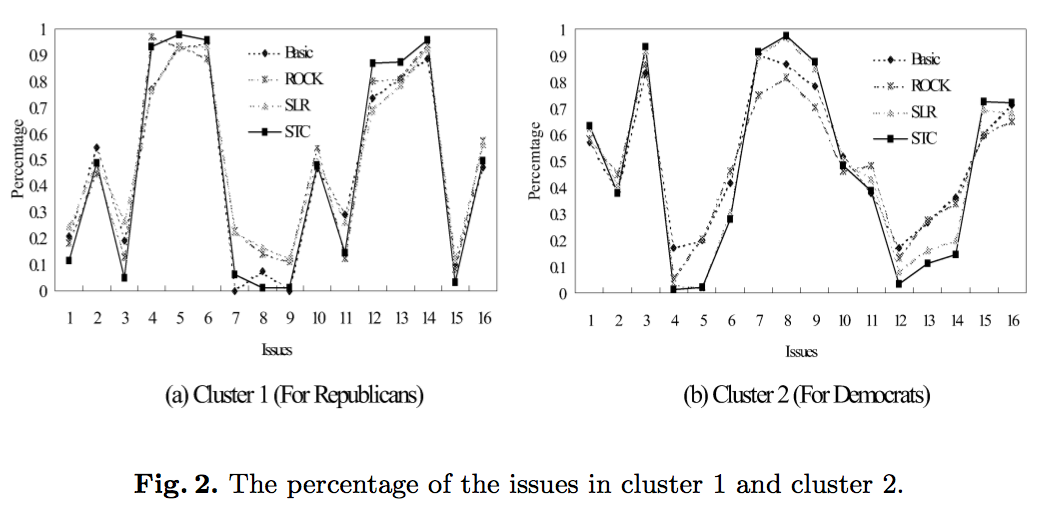
\includegraphics[scale=.75]{pic2}

From the data of the experiment we can see that STC has the best clustering quality in most issues ($\frac{22}{32}$ or 69$\%$)

\subsection{Experiment Three: Evaluating the scalability by synthetic workload.} This experiment is meant to show how well each algorithm performs as the number of transactions varies from 5000 to 20000. The number of items $N^I$ is set to 1000 and the size of the transaction is picked from a Poisson distribution with mean $|T| = 5$. The data shows that algorithm STC outperforms all other algorithms in scalability. As the number of transactions increases, algorithm STC's execution time grows the slowest.

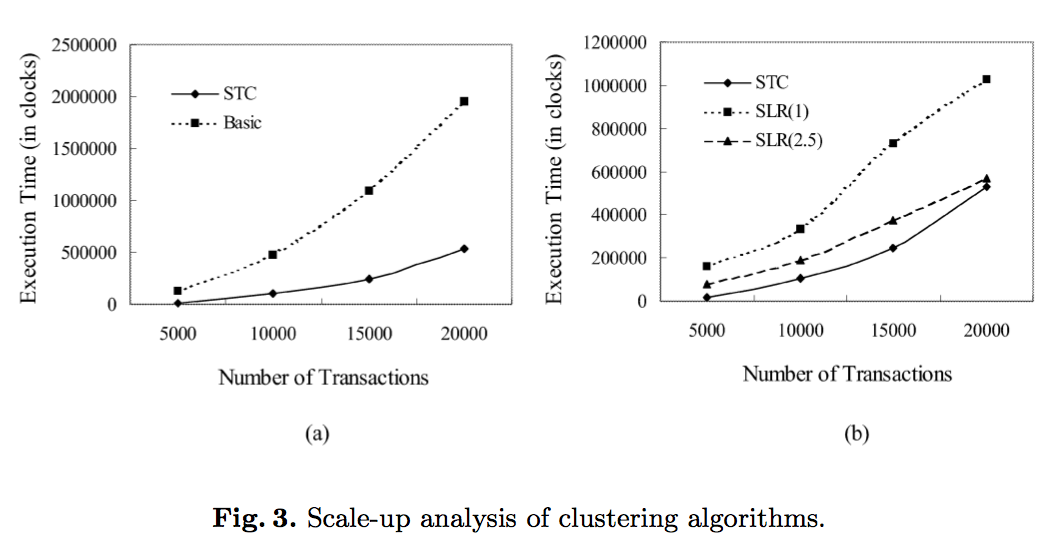
\includegraphics[scale=.75]{pic3}

%==================================
\section{Conclusion}
%==================================

Algorithm STC utilizes a self-tuning technique for adaptively tuning the input and output SL ratio thresholds to minimize the SL ratios of transactions in the clusters efficiently. By utilizing the self-tuning technique, algorithm STC is able to efficiently minimize the SL rations of transactions in the clusters. Several experiments were conducted to compare STC with other similar clustering algorithms.  It is shown in the results of the experiments that using the self-tuning technique in STC allows the STC algorithm to outperform algorithm SLR, algorithm ROCK and algorithm STC without self-tuning. Algorithm STC not only outperforms the others in execution time but also provides the best quality clusters.

The end

\end{document}



